The model describes a core composed of hexagonal graphite assemblies Figs. \ref{fig:FullXY} and \ref{fig:FullYZ} of 30 cm (flat-to-flat).  different types assemblies make up the core, the fuel assembly Fig. \ref{fig:FuelAssembly}, the control rod assembly Fig. \ref{fig:ControlRodAssembly}, and a central assembly Fig. \ref{fig:CentralAssembly}. The fuel assembly consists of 54 fuel channels and 19 cooling channels. The control rod assembly hosts the control rod guide (8 cm-diameter) and consists of 48 fuel channels and 18 cooling channels. The central assembly has one 12 cm-diameter control rod \cite{hawari_development_2018}. The fuel channels are 2 cm diameter. The fuel compacts are 1.4 cm diameter. The fuel channel wall and the compacts have a 0.3 cm gap filled with He. The cooling channels are 1.45 cm diameter. The core has a top and bottom reflector of graphite. The hexagonal core as a radial reflector of graphite and another one of BeO.

\begin{figure}[H]
	\centering
	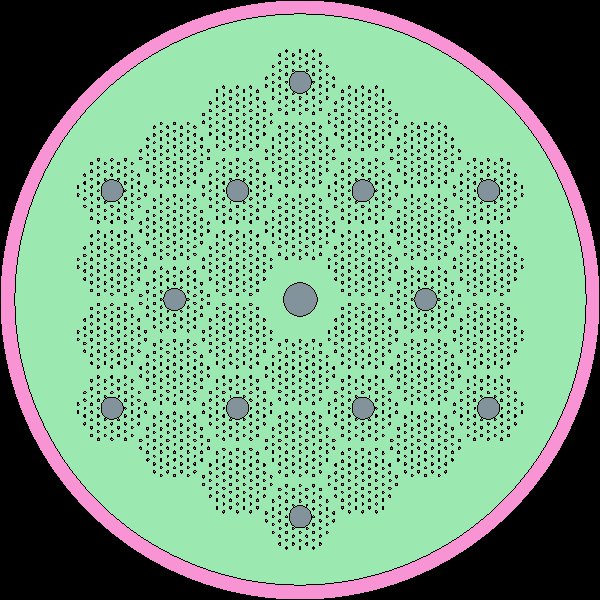
\includegraphics[width=0.45\linewidth]{figures/MMR_full_stack_geom1.png}
	\hfill
	\caption{XY cross section of the full core Serpent2 model geometry.}
	\label{fig:FullXY}
\end{figure}

\begin{figure}[H]
	\centering
	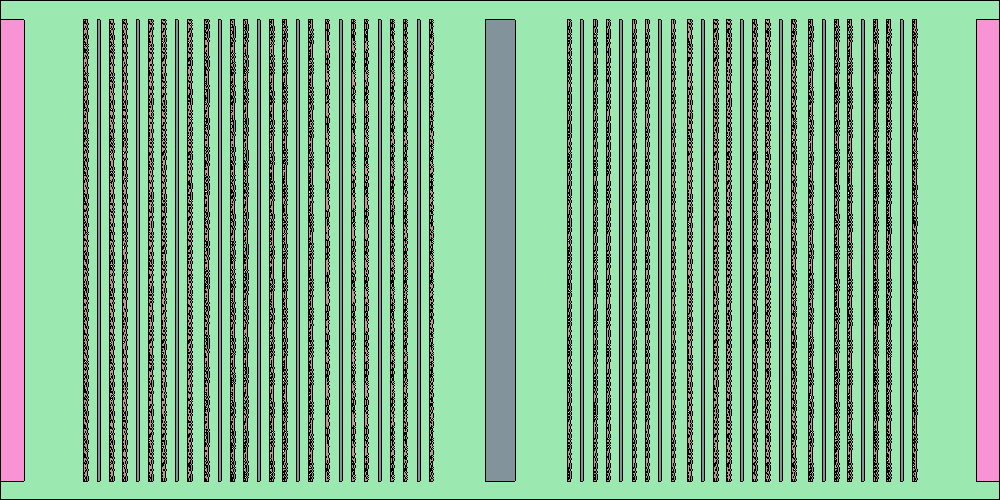
\includegraphics[width=0.6\linewidth]{figures/MMR_full_stack_geom2.png}
	\hfill
	\caption{YZ cross section of the full core Serpent2 model geometry.}
	\label{fig:FullYZ}
\end{figure}

\begin{figure}[H]
	\centering
	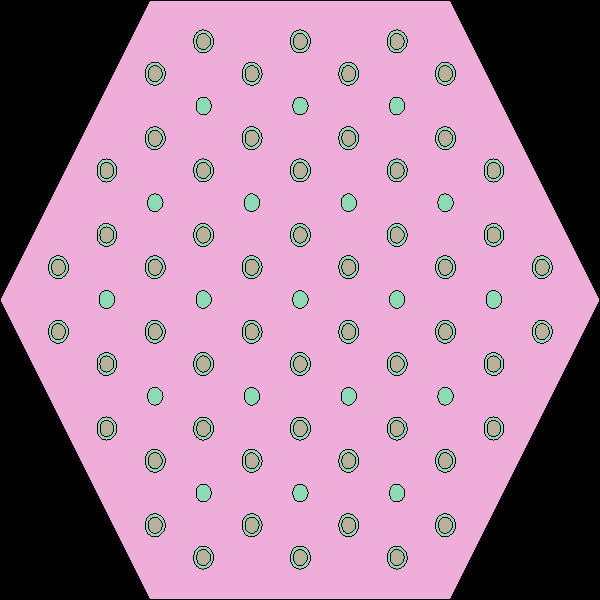
\includegraphics[width=0.4\linewidth]{figures/fuel_block_geom1.png} 
	\hfill
	\caption{Fuel Assembly Serpent2 model geometry.}
	\label{fig:FuelAssembly}
\end{figure}

\begin{figure}[H]
	\centering
	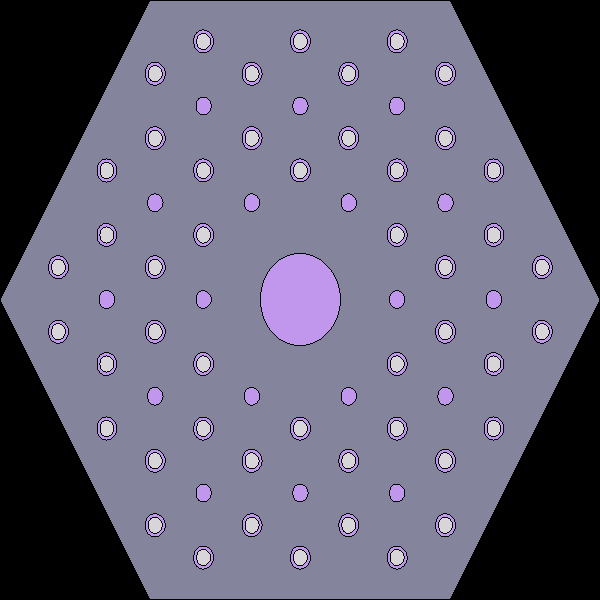
\includegraphics[width=0.4\linewidth]{figures/control_block_geom1.png} 
	\hfill
	\caption{Control Rod Assembly Serpent2 model geometry.}
	\label{fig:ControlRodAssembly}
\end{figure}

\begin{figure}[H]
	\centering
	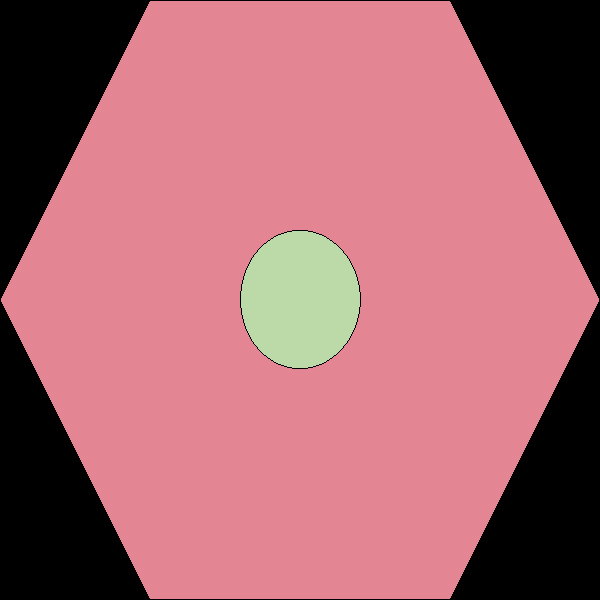
\includegraphics[width=0.4\linewidth]{figures/central_block_geom1.png}
	\hfill
	\caption{Central Assembly Serpent2 model geometry.}
	\label{fig:CentralAssembly}
\end{figure}

\section{Results}

Both cases use 100 active cycles and 40 inactive cycles. The number of particles is 5000 for each cycle.

The eigenvalue of an elementary cell containing a fuel channel (Fig. \ref{fig:FCM}) is: \\
\noindent
k-eff (analog)    = 1.40963 +/- 0.00164  [1.40641  1.41284]\\
\noindent
k-eff (implicit)  = 1.41108 +/- 0.00090  [1.40932  1.41285]

The eigenvalue of the full core (Fig. \ref{fig:FullXY}) results:\\
\noindent
k-eff (analog)    = 0.79770 +/- 0.00193  [0.79392  0.80148]\\
\noindent
k-eff (implicit)  = 0.79688 +/- 0.00156  [0.79383  0.79993]